\documentclass[conference,final]{IEEEtran}

\usepackage{latex8}
\usepackage{times}

\usepackage[utf8]{inputenc}
\usepackage{graphicx}
\usepackage{url}
\usepackage{float}
\usepackage{times}    
\usepackage{multirow}    
\usepackage{listings}   
\usepackage{times}     
\usepackage{paralist}    
\usepackage{wrapfig}    
\usepackage[small,it]{caption}
\usepackage{multirow}
\usepackage{ifpdf}
\usepackage{srcltx}


\usepackage{listings}
\usepackage{keyval}  
\usepackage{color}
\definecolor{listinggray}{gray}{0.95}
\definecolor{darkgray}{gray}{0.7}
\definecolor{commentgreen}{rgb}{0, 0.4, 0}
\definecolor{darkblue}{rgb}{0, 0, 0.4}
\definecolor{middleblue}{rgb}{0, 0, 0.7}
\definecolor{darkred}{rgb}{0.4, 0, 0}
\definecolor{brown}{rgb}{0.5, 0.5, 0}

\lstdefinestyle{myListing}{
  frame=single,   
  backgroundcolor=\color{listinggray},  
  %float=t,
  language=C,       
  basicstyle=\ttfamily \footnotesize,
  breakautoindent=true,
  breaklines=true
  tabsize=2,
  captionpos=b,  
  aboveskip=0em,
  belowskip=-2em,
  %numbers=left, 
  %numberstyle=\tiny
}      

\lstdefinestyle{myPythonListing}{
  frame=single,   
  backgroundcolor=\color{listinggray},  
  %float=t,
  language=Python,       
  basicstyle=\ttfamily \footnotesize,
  breakautoindent=true,
  breaklines=true
  tabsize=2,
  captionpos=b,  
  %numbers=left, 
  %numberstyle=\tiny
}

\newcommand{\up}{\vspace*{-1em}}
\newcommand{\upp}{\vspace*{-0.5em}}
\newcommand{\numrep}{8 }
\newcommand{\samplenum}{4 }
\newcommand{\tmax}{$T_{max}$ }
\newcommand{\tc}{$T_{C}$ }
\newcommand{\tcnsp}{$T_{C}$}
\newcommand{\bj}{BigJob}

% \title{Running Molecular Dynamics Ensembles and Replica-Exchange
%   Simulations on Azure} 
%\title{Patterns for Pleasingly Parallel Bio-molecular Simulations on
%Azure}

\title{Abstractions for Loosely-Coupled and Ensemble-based Simulations
  on Azure\up}

\author{
Andr\'e Luckow$^{1}$, Shantenu Jha$^{1,2,3,*}$\\
  \small{\emph{$^{1}$Center for Computation \& Technology, Louisiana State University, USA}}\\
  \small{\emph{$^{2}$Department of Computer Science, Louisiana State University, USA}}\\
  \small{\emph{$^{3}$e-Science Institute, Edinburgh, UK}}\\
  \small{\emph{$^{*}$Contact Author: \texttt{sjha@cct.lsu.edu}}}\\
  \up\up\up\up
}

%\date{}

\def\acknowledgementname{Acknowledgements}
\newenvironment{acknowledgement}%
{\section*{\acknowledgementname}%
\parindent=0pt%
}

\newif\ifdraft
%\drafttrue
\ifdraft
\newcommand{\llnote}[1]{ {\textcolor{green} { ***JK: #1 }}}
\newcommand{\alnote}[1]{ {\textcolor{blue} { ***AL: #1 }}}
\newcommand{\jhanote}[1]{ {\textcolor{red} { ***SJ: #1 }}}
\else
\newcommand{\llnote}[1]{}
\newcommand{\alnote}[1]{}
\newcommand{\jhanote}[1]{}
\fi

\begin{document} 

\maketitle    

\begin{abstract}
  Azure is an emerging cloud platform developed and operated by
  Microsoft.  It provides a range of abstractions and building blocks
  for creating scalable and reliable scientific applications.  In this
  paper we investigate the applicability of the Azure abstractions to
  the well-known class of loosely coupled and ensemble-based
  applications.  We propose the BigJob API as a novel abstraction for
  managing groups of Azure worker roles and for remotely executing
  tasks on them. We demonstrate that Azure enhanced with BigJob
  functionality provides performance comparable to other grid and
  cloud offerings loosely-coupled applications.  \up \up

\end{abstract}
\section{Introduction}
\up
% Distributed infrastructures have been used by many applications to
% advance understanding in their disciplines. Clouds as represented by
% Microsoft’s Azure Platform are emerging as an important class of
% distributed computational resources, for both data-intensive and
% compute-intensive applications. 
Emerging cloud platforms such as Microsoft's Azure~\cite{winazure},
present relatively simple computing environments compared to
traditional grid computing environments, in terms of resource
management, capacity planning capabilities, software environment \&
control etc. % \alnote{don't quite understand this first sentence}
% \jhanote{Is this better?} \alnote{yes}
In spite of the promise of clouds as a
viable platform for Science \& Engineering applications, many
fundamental questions persist about how scientific applications will
utilize clouds as presented, both now and into the future? Some
existing legacy applications no doubt will adapt and take advantage of
new capabilities, but it is unclear how clouds as currently presented
are likely to change (fundamentally?)  the development and deployment
of scientific applications, and the process of scientific
investigation. The challenges surrounding the effective uptake of
clouds are both broad and deep, in that, there are both
application-level questions as well as system-level questions.  For
example, are clouds viable alternatives to production grid
infrastructure or will they be part of a larger production
cyberinfrastructure? What kind of scientific services can clouds
support and how should clouds be provisioned and provided to the
scientific community?

% do clouds present, 

% For example, what kind of CI do clouds present, and how should clouds
% be provisioned and what services should be provided to the scientific
% community?

% \jhanote{The aim of this paper is to  explore... integrate..fill... particularly arises as a consequence}  
% \alnote{don't understand the first part of the sentence.}
% \jhanote{Sorry -- this was a note to myself. I'll fix} 
 


% The aim of this paper is to explore the
% Azure cloud platform.

% In contrast to infrastructure as a service
% clouds (IaaS) as Amazon EC2/S3, Azure follows the platform as a
% service paradigm (PaaS).  The platform encapsulates common application
% patterns into so-called roles removing the need to manually manage
% low-level details on virtual machine level.

% \alnote{not sure whether we should explain the difference to IaaS -
%   space is tight} \jhanote{Probably not}

 
% Cloud are posed to have a broad impact on scientific applications, as
% they provide novel and exciting opportunities for Science \&
% Engineering Applications (SEA). 

% how clouds -- particularly the Azure platform -- can support
% scientific applications in the domain of molecular dynamics.

% by simply performing the same simulation repeatedly (enD).  More
% demanding are ensembles of coupled simulations: 

To understand some of these questions we investigate Ensemble-based
(enMD) approaches, which are commonly used in simulations to
facilitate drug discovery and to provide fundamental insight into
molecular structure, dynamics and interactions.  Different kinds of
ensemble-based approaches are commonly deployed: Ensembles of
independent simulations aim to improve the statistical sampling of MD
simulations.  In some scenarios, sampling of physical-states can be
improved by infrequent attempts to exchange partial state information
between pairs of replicas; the replica-exchange (RE)
algorithm~\cite{hansmann} is a well-known example of this class.

In Luckow et\,al.~\cite{repex_ptrsb} efficient scale-out of RE
simulations was established for multiple TeraGrid (TG) resources. We
used the BigJob framework to decouple workload submission from
resource assignment; this results in a flexible execution model, which
in turn enables the distributed scale-out of applications on multiple
and possibly heterogeneous resources {\it concurrently}.  In
Ref.~\cite{10.1109/CCGRID.2010.91} we extended this work to support
production grid infrastructures based on Condor as well as EC2-style
clouds (e.\,g.\ FutureGrid).
 
% This is not a research paper, but an experience and experiment
% paper. 
The primary aim of this paper is to explore the abstractions that the
Windows Azure platform provides, and their suitability to for
orchestrating distributed, loosely-coupled workloads, as required by
enMD simulations. Furthermore, we determine how existing and
established abstractions for distributed computing can be extended to
Azure.  We analyze the suitability of the different Azure
abstractions, such as the Azure Queue-service (AQS), Azure Blob
Storage (ABS) and the Worker Role API.% we find that they
We propose the existing BigJob API as an viable and efficient
abstraction for managing a group of Azure worker roles and for
remotely executing tasks on them.

% provide powerful tools for orchestrating distributed workloads, as
% required by enMD simulations.  

% Based upon our research choose as our with respect to the enMD and
% REMD use case.  \jhanote{Given that we're not using SAGA BigJob
%   here, should we call this an extension of the earlier work?}

% We show that Azure abstractions, such as the Azure Queue and ABS as
% well as the Worker Role API, provide powerful tools for orchestrating
% distributed workload as found in the RE use case. 

% The proposed framework will encapsulate Azure specifics so that the
% REMD and enMD use cases can easily ported to Azure.


This paper is structured as follows: In \S~\ref{sec:azure} we present
an overview of the Azure platform. In \S~\ref{sec:pilot-bj} the pilot-job 
concept and the BigJob framework is introduced. The Azure BigJob 
implementation is presented in \S~\ref{sec:bigjob-saga}.
In \S~\ref{sec:enMD-REMD} we discuss the
architecture of the Azure-based enMD and RE application.  A
significant issue in cloud computing is performance. We provide an
in-depth performance analysis in \S~\ref{sec:performance}.

% \section{Related Work}
% \up \alnote{Do we need related work? Or are our references
%   sufficient?}  AzureBlast~\cite{azure_blast} \jhanote{I think
%   references are good enough. I don't know if there is a
%   protocol/space-economics of a 4page paper..}
\up
\section{Windows Azure}
\label{sec:azure}
\up
% Azure provides different higher level services, e.\,g.\ the Azure
% AppFabric or Azure Storage, that can be accessed via HTTP/REST from
% anywhere. 
Windows Azure offers a platform for on-demand computing and for
hosting generic server-side applications.  In contrast to
infrastructure as a service clouds (IaaS), such as Amazon EC2/S3,
Azure follows the platform as a service paradigm (PaaS).  The platform
encapsulates common application patterns into so-called {\it roles},
removing the need to manually manage low-level details on virtual
machine (VM) level.  The so-called Azure fabric controller
automatically monitors all VMs, reacts to hardware and software
failures and manages application upgrades.

\subsubsection{Compute}

Windows Azure currently provides two kind of 
roles: Web roles e.\,g.\ are used to host web applications and
front-end code, while worker roles are well suited for background
processing. While these roles target specific scenarios and are not as
flexible as bare EC2 images, they are also customizable, % to a certain
% extent,
e.g., Worker roles can run native code. The application must implement
the worker role API, which provides a \texttt{run} method as a defined
entry point for executing the actual compute task. Further, several
additional API callbacks, e.\,g.,\ for state or configuration change
notifications, are provided.%
% \jhanote{This is a bit unclear to the reader: What is an 'entry point'
%   here..? What is important about an application 'must soley
%   implement' it?} \alnote{added some more worker role API background}
The Azure fabric controller automatically manages and monitors
applications, handles hardware and software failures as well as
updates to the operating system or the application.  Scientific
applications commonly utilize worker roles for compute and/or
data-intensive tasks. AzureBlast~\cite{azure_blast} e.\,g.\ heavily
relies on worker roles for computing bio-sequences.

\subsubsection{Storage}

Azure provides three key services or storing large amounts of data:
the \emph{Azure Blob Storage} (ABS) for storing large objects of raw
data; the \emph{Azure Table Storage} (ATS) for semi-structured data,
and the \emph{Azure Queue Storage} (AQS) for implementing message
queues.  The stored data is % storage
replicated across multiple data centers to protect it against hardware
and software failures. In contrast to other services (e.\,g.\ Amazon
S3)~\cite{1294281}, the Azure Storage Services provide strong
consistency guarantees, i.\,e.,\ all changes are immediately visible to
all future calls. While eventual consistency offers a better
performance and scalability, it has some disadvantages mainly caused
by the fact that the complexity is moved to the application space.

ABS can store file up to a size of 1\,TB, which makes it particularly
well suited for data-intensive applications. S3 e.\,g.\ restricts the
maximum file size to 5\,GB. Further, the access to the ABS blob
storage can be optimized for certain usage modes: \emph{block blob}
can be split into chunks which can be uploaded and downloaded
separately and in parallel.  Thus, block blobs are well suited for
large amounts of data. \emph{Page blob} manage the storage as an array
of pages. Each of these pages can be addressed individually, which
makes page blobs a good tool for random read/write scenarios.

% \emph{Azure XDrive} provides a durable
% NTFS volume, which is backed by a page blob. In particular legacy
% applications that heavily utilize file-based storage can simply be
% ported to Azure using XDrive.

AQS provides reliable storage for the delivery of messages for
distributed applications.  It is ideal to orchestrate the various
components of a distributed application, e.\,g.\ by distributing work
packages or collecting results.
%, which could be running on Azure or on another resource,
%e.\,g.\ the TeraGrid.

% The Azure Table Storage is ideally suited for storing structured
% data. Unlike traditional relational database systems, the table
% storage is designed with respect to scale-out, low cost and high
% performance similar to Google's BigTable~\cite{bigtable2006}
% system. For legacy application Azure also provides a SQL-Server based,
% relational datastores called SQL Azure. In contrast to Azure tables,
% SQL storage supports common relation database features, such as
% foreign keys, joins and SQL as query language.
% \alnote{removed Azure components that are not used by
%   REMD}\jhanote{OK}

\up
\section{Pilot-Jobs and SAGA BigJob}
\label{sec:pilot-bj}
\up

Pilot-Jobs are a useful abstraction for efficiently executing an
ensemble of batch jobs on distributed infrastructures without the
necessity to queue each individual job.  The pilot-job itself is a
regular grid job, which is started through a grid resource manager,
such as the Globus GRAM.  Once the batch queue assigns the requested
resources to the pilot-job, the pilot-job circumvents the necessity to
queue each individual sub-job, and is responsible for managing the
resources.  Thus queuing times for sub-jobs can be reduced and the
predictability for application execution can be increased. In effect,
pilot-jobs decouple resource allocation from resource binding and
allow the efficient utilization of resources. By delaying the resource
binding, and enabling scheduling decision at the application-level,
dynamic execution and usage modes can be supported.  For example, the
load-dependent sizing of sub-jobs, or the dynamic addition of
resources to meet deadlines~\cite{10.1109/CCGRID.2010.91}.

As more applications take advantage of dynamic execution, the
pilot-job concept has grown in popularity and has been extensively
researched and implemented for different usage scenarios and
infrastructure including clouds.  Nimbus~\cite{10.1109/MIC.2009.94}
e.\,g. provides a pilot-job like abstractions for clouds. For this
purpose, Nimbus allows the launch of auto-configured virtual machine
clusters that contain a Torque and Globus installation.  The Atlas
computing framework developed at CERN also heavily relies on the PanDA
pilot-job framework~\cite{1742-6596-219-6-062041} to implement
resource leases. Using the VIRM API, PanDA was extended to support
different virtualization backends, e.\,g.\ OpenNebula and Nimbus. Both
frameworks are strongly coupled to a particular backend infrastructure
-- Globus in the case of Nimbus and gLite in the case of PanDA. The
advantage of the SAGA pilot-job is that it allows applications to
seamlessly utilize different backend infrastructure, e.\,g.\ Condor,
Globus and different kinds of clouds, at the same time.

SAGA~\cite{saga_url} is a simple, POSIX-style API to the most common
distributed functions, which is a sufficiently high-level of
abstraction so as to be independent of the diverse and dynamic grid
environments.  \emph{BigJob} is a SAGA-based pilot-job
implementation~\cite{10.1109/CCGRID.2010.91}, which can, in contrast
to other pilot-job implementations, natively works independent of the
underlying distributed infrastructure and across different
heterogeneous backend, e.\,g.\ grids, Condor pools as well as
EC2-based and Azure clouds, reflecting the advantage of using a
SAGA-based approach (see
Figure~\ref{fig:figures_distributed_pilot_job}). Furthermore, the
framework is extensible and provides several hooks that can be used to
support other resource types, pilot-job frameworks and
application-specific customization.

\begin{figure}[ht]
    \centering
    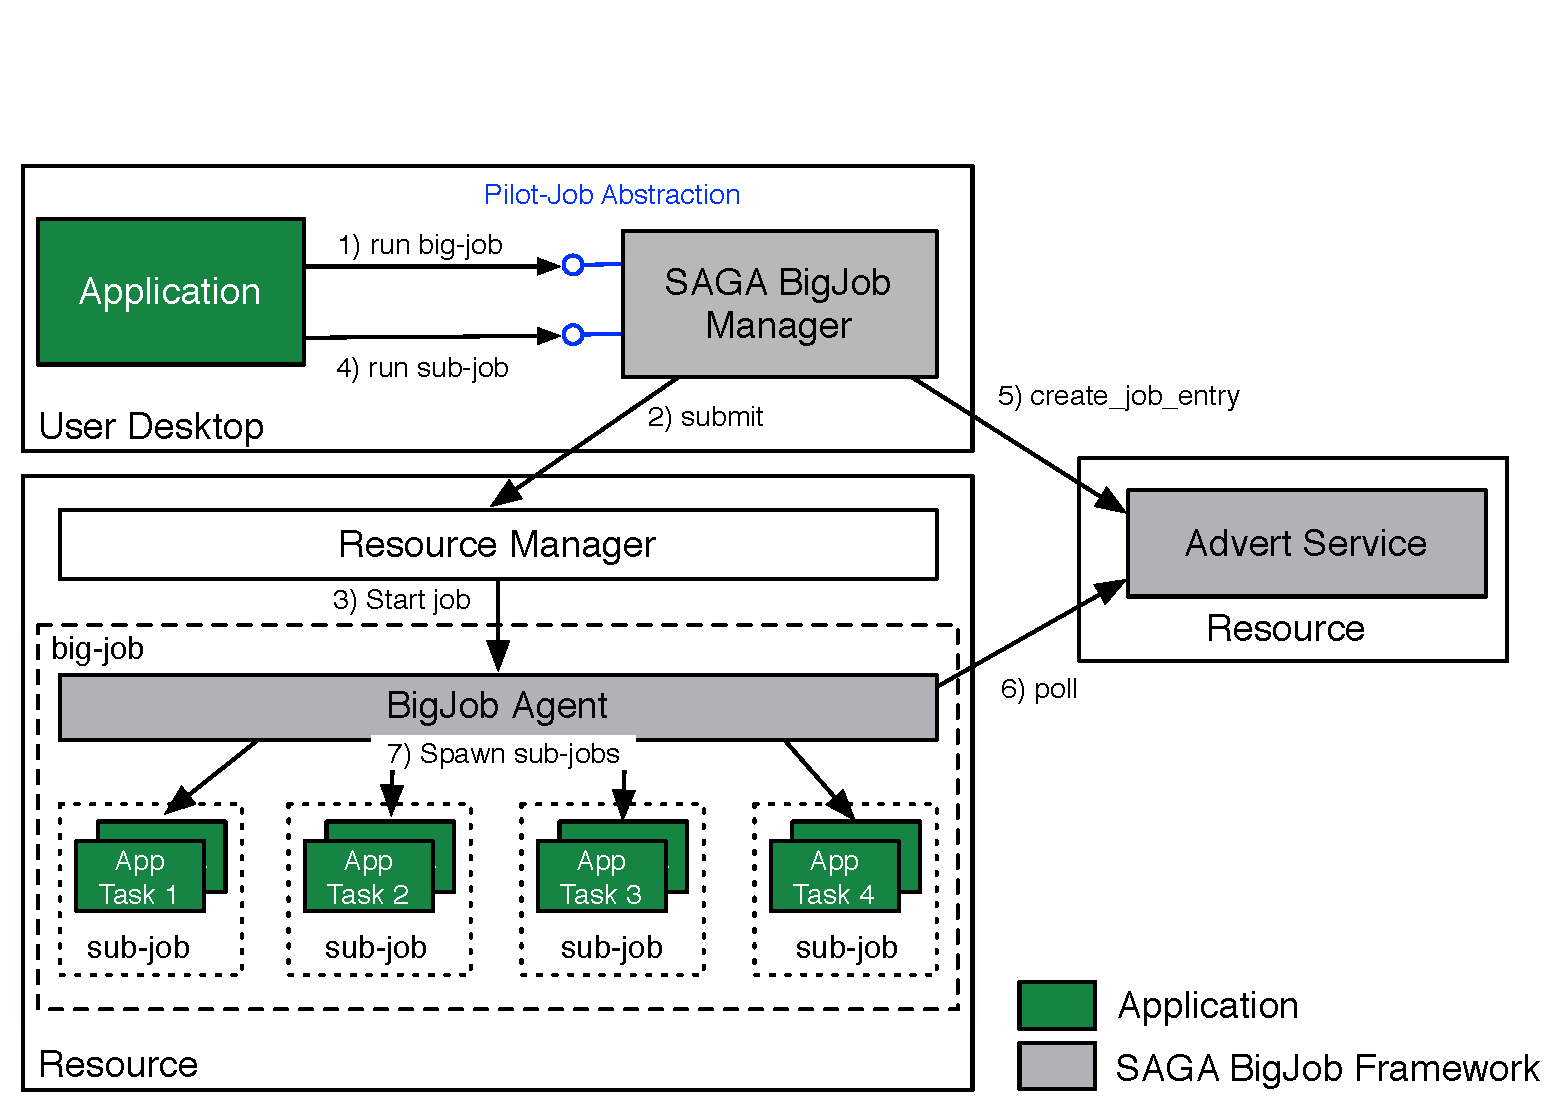
\includegraphics[width=0.45\textwidth]{figures/bigjob}
   \caption{BigJob Architecture: The core of the framework, the
      BigJob Manager, orchestrates a set of sub-jobs via a
      BigJob Agent using the SAGA job and file APIs.  The
      BigJob Agent is responsible for managing and monitoring sub-jobs.\up}
   \label{fig:figures_bigjob}   
\end{figure}

Figure~\ref{fig:figures_bigjob} shows an overview of the SAGA BigJob
implementation for computational grids. The grid BigJob comprises of
three components: (i) the BigJob Manager (BM) that provides the
pilot-job abstraction to the application, and manages the
orchestration and scheduling of BigJobs (which in turn allows the
management of both big-job objects and sub-jobs), (ii) the BigJob
Agent (BA) that represents the pilot-job, and (iii) the advert service
which is used for communication between the BM and BA.
% \jhanote{Andre, the third
%   component, or at least (iii) is missing!}\alnote{fixed}

Applications can utilize the framework via the big-job and sub-job
classes. Both interfaces are syntactically and semantically consistent
with the other SAGA APIs: a sub-job for example, is described using
the standard SAGA job description; job states are expressed using the
SAGA state model. Before running sub-jobs, an application must
initialize a big-job object. The BM then queues a job, which actually
runs a BigJob Agent on the respective remote resource. For this agent
a specified number of resources is requested. Subsequently, sub-jobs
can be submitted through the BM using the job-id of the BigJob as
reference. The BM ensures that sub-jobs are launched onto the correct
resource based upon the specified job-id using the right number of
processes.

% The BigJob API is a SAGA-style API that utilizes common SAGA idioms
% and classes (e.\,g.\ saga.job.description) for managing pilot-jobs and
% for starting sub-jobs.  



\up
\section{Azure BigJob}
\label{sec:bigjob-saga}
\up

% \emph{BigJob} is a infrastructure-independent
% pilot-job implementation~\cite{10.1109/CCGRID.2010.91}.  As shown in
% Figure~\ref{fig:figures_distributed_pilot_job}, BigJob provides a
% unified abstraction to grids, Condor pools, EC2-style clouds and to
% Windows Azure. Using the same API, applications can dynamically
% allocate resources via the big-job interface and bind sub-jobs to
% these resources.

\begin{figure}[t]
    \centering
        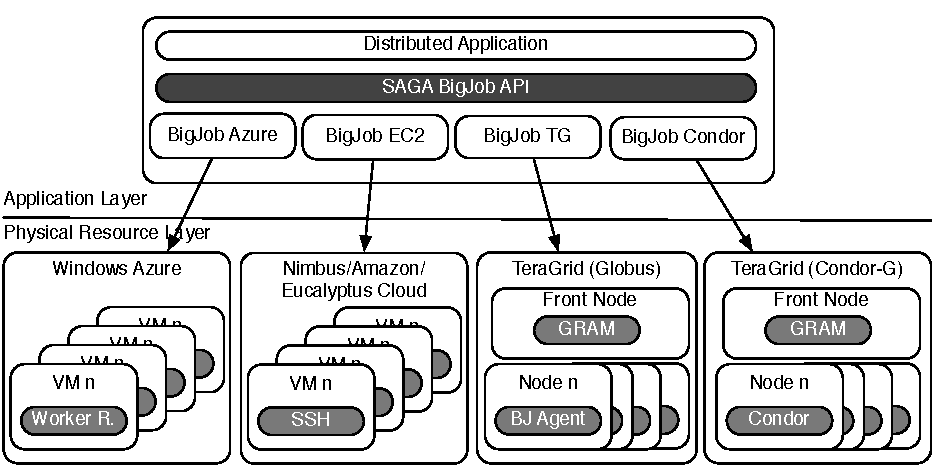
\includegraphics[width=0.42\textwidth]{figures/distributed_pilot_job}
        \caption{\textbf{Overview of the BigJob Architecture:} BigJob
          can currently be used with four different infrastructures:
          grids, Condor pools, EC2-style and Azure clouds.\up}
    \label{fig:figures_distributed_pilot_job}
\end{figure}

Figure~\ref{fig:figures_bigjob_azure} illustrates the architecture of
the Azure-based BigJob. Similarly to the grid BigJob BM, the Azure BM
is responsible for accepting simulation requests from the end-user and
for orchestrating the sub-job runs.  In contrast, to the grid BigJob,
which utilizes different packages of the SAGA API~\cite{saga_url}, the
Azure BigJob is built directly on top of the Azure APIs. With the
exception of using the BigJob API -- and thus presenting an interface
that is identical to the SAGA-based pilot-job and that which is used
for other infrastructures, Azure BigJob is self-contained and
independent of any (SAGA) details used to implement a SAGA-based
pilot-job.


Initially, the BM launches the requested number of worker
roles % (also referred to
% as VM) 
using the Service Management API -- a RESTful HTTP API.
%The Service Management API is a RESTful HTTP API
As part of this project we developed a Python library that can be used
to access this Azure capability~\cite{azure-service-python}. The
BigJob Agents run within the worker roles and are implemented in
C\#/.NET. The main responsibility of the agent is to execute the
specified MD code, (e.\,g.\ NAMD~\cite{Phillips:2005gd}, or
AMBER~\cite{tec2}), on the worker. Azure restricts communication
between worker roles to a set of pre-defined endpoints.
% \jhanote{something missing..}\alnote{hopefully better now}
Since MPI utilizes dynamically assigned ports, MPI computations cannot
be run across multiple worker roles.  The size of a parallel
simulation is therefore limited to the VM size (the largest Azure VM
has currently 8 cores).

For each sub-job the BM creates a work-package. These are distributed
to the agents using the AQS, which by offering a reliable and scalable
way for delivering messages to distributed components, provide an
ideal abstraction. These can, but do not have to be hosted on Azure.



%%%%%%%%%%%%%%
% \jhanote{I am a bit confused about if we're using BigJob-Azure in
%   conjuction with other BigJob agents, i.e i.e., SAGA-BigJob API is
%   used, but not SAGA in the execution?  Is this correct?}  \alnote{The
%   Azure BigJob is completely self-contained and has nothing in common
%   with the SAGA BigJob except the API. Hope this gets clearer once I
%   remove the SAGA BigJob stuff.}\jhanote{Yes, it reads better. But
%   please leave this comment on for a while. Want to revisit it later}

%-- it ensures atomicity and an at least once semantic --
% \jhanote{this sub-clause needs attention.. something amiss}
% \alnote{removed clause}%

% The SAGA-based BigJob in contrast utilizes
% the SAGA advert service, a central key/value store, for this purpose. 
% For each new job, an advert entry is created by the BigJob Manager. 
% The agent periodically polls for new jobs. Azure Queues provide a higher
% level of abstractions ensuring atomicity and an at least once semantic.

%\begin{wrapfigure}{R}{0.4\textwidth}
\begin{figure}
    \centering
    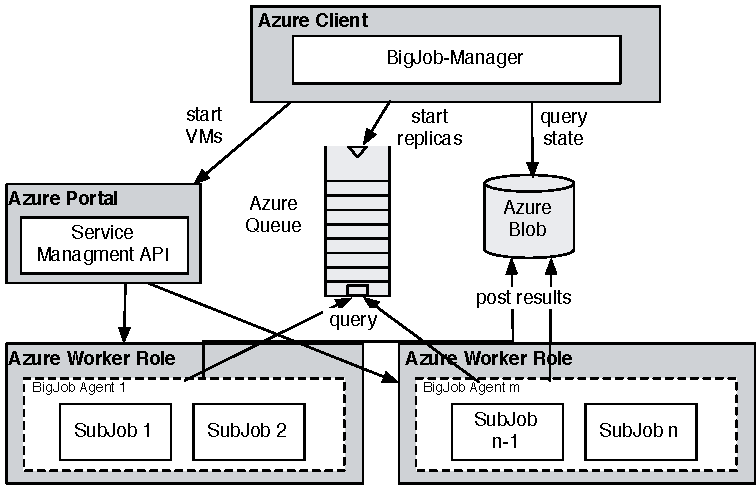
\includegraphics[width=.4\textwidth]{figures/bigjob_azure}
    \caption{\textbf{Azure-based BigJob:} The framework
      utilizes the queue storage for distributing work
      packages from the BigJob Manager to the
      BigJob agents running on multiple worker roles.}
    \label{fig:figures_bigjob_azure}
    \up\up
\end{figure}

Once the agents are started, they query the AQS for new work packages.
If a package is found, a simulation task is started, e.\,g.\ by
running the requested MD code with right parameters. The framework
supports both the staging of parameter files as well as of the
executable using ABS. If staging is requested in the job description, 
the manager uploads the respective files
to the storage and the agents downloads them before the run.

The framework supports Azure affinity groups.  % \jhanote{Can you
%   clarify which kinds of affinity are supported?}  \alnote{added a
%   sentence}
%which can be used to co-locate compute tasks and storage. 
If requested, BigJob uses affinity groups to place the VMs for the
sub-jobs and the Azure storage for file staging close to each other in
the same data center.  This is particularly useful for data-intensive
tasks, e.\,g.\ MapReduce applications. At the same time the BM can
also orchestrate worker roles that are distributed across multiple
affinity groups.


% The worker roles running the BigJob agent are managed by the BigJob Manager using
% the Azure Service Management API. In the initial version we will
% support the automatic start and stop of hosted services. In the final
% version there will be a possibility to automatically deploy agent code
% without the need to pre-configuring the VMs. 


% \alnote{Kalman Filter option: we need to convey how we make decisions?
% we need to understand the various trade-offs}
\up
\section{EnMD and RE Simulations on Azure}
\label{sec:enMD-REMD}
\up Using the BigJob framework we have deployed and executed both the
independent and coupled ensemble scenarios (enMD \& REMD).  Both
scenarios utilize the BigJob API to create pilot-jobs, and
subsequently to submit sub-jobs. When a pilot-job is created the
BigJob framework initializes the requested number of worker roles with
the specified size and launches a virtual cluster of Azure
workers. The replicas themselves are submitted as sub-jobs.  After the
sub-job terminates, the application can
collect results via the BigJob API.  NAMD is used to perform MD
simulations.  In the REMD case the output is parsed to obtain the
energy level of the replica.  The Metropolis scheme is used to
determine whether an exchange is accepted. Finally, a new generation
of replicas is launched.

% The sub-jobs per worker role depends on the size of the worker role
% -- Azure currently supports worker roles up to 8 cores. In contrast
% to other infrastructure types such as EC2 and the TeraGrid, MD jobs
% cannot be spawned across multiple nodes.

% Both enMD and REMD can greatly benefit from the capabilities of
% Azure. If greater accuracy is required or a deadline must be met, it
% can seamlessly scale-out to more worker roles.  The Azure fabric
% controller monitors all VMs running the worker roles and
% automatically restarts the worker roles if necessary. Further, Azure
% provides various kinds of reliable and scalable storage options to
% express different coordination schemes, e.\,g.\ the master-worker
% communication can be conducted via the described message queue.


\up
\section{Performance Analysis}
\label{sec:performance}
\up The aim of this section is not to perform detailed systematic
performance measures and analysis, but to illustrate the
representative usage modes BigJob can support, and to explain how they
are supported.  % We discuss two scenarios\jhanote{Can we illustrate
% which two scenarios please?} that are representative of how
% applications would typically use multiple distributed
% infrastructures.
We focus our attention on RE MD-simulations, and a workload of \numrep
replicas of a Hepatitis-C virus (HCV) model, with each replica running
for 500 timesteps.  \up

\subsection{BigJob Startup Times}
\up Initially, we analyze the overhead resulting from the usage of
BigJob across different infrastructures. Typically, the main overhead
when using BigJob results from either the queueing time at individual
resources for grids or from the VM creation time for cloud
environments.  Figure~\ref{fig:performance_setup_time} compares the
average startup times of the different BigJob
backends % \jhanote{should
%   we use BigJob backend in lieu of pilot-job backend here?}
% \alnote{Makes sense. Replaced it.}
for grids, Condor pools and clouds. Each experiment was repeated at
least 10 times.

\begin{figure}[htbp]
    \centering
        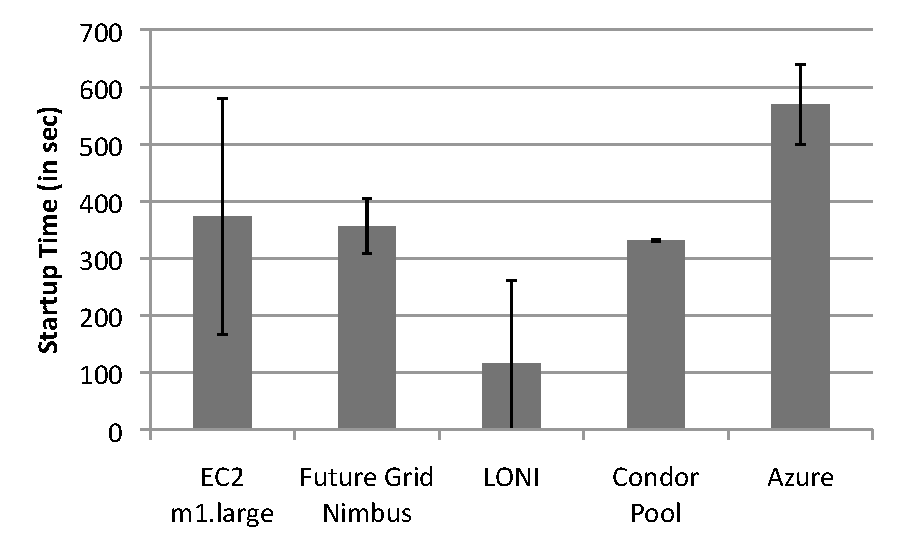
\includegraphics[width=0.4\textwidth]{performance/setup-times}
    \caption{\textbf{BigJob Startup Times:} In grids the startup time
      greatly depends upon the queuing time at the local resource
      manager. However, in our experiments also clouds showed a high
      fluctuation in the queueing time. Azure shows a slightly higher
      startup time than the science and the EC2 clouds.\up}
    \label{fig:performance_setup_time}
\end{figure}

Interestingly for experiments conducted,  startup times for the
cloud environments were observed to be larger than the queue waiting
time for the LONI resource Poseidon. % \jhanote{which coincidentally was
%   very lightly loaded during the course of these experiments.}
% \alnote{agree, this part can be removed.} 
Obviously, the startup of a VM involves higher overheads than spawning
a job on an already running machine: a resource for the VM must be
allocated, the VM must be staged to the target and booted up. The data
show that
% also show that especially
the already over-subscribed intra-cloud network and thus, the staging
of the VM can be a bottleneck. Azure VMs had the longest waiting time
($>10$\,min; about 200\,sec longer than EC2).
%which is consistent with Hill et\,al.~\cite{hill10}.  
Further, high fluctuations in waiting times can be observed. These
waiting time usually correlate to the current load of the chosen data
center, which again depends on external factors, such as the location
of the data center and/or the date/time of the request.

BigJob can manage sets of VMs, and thus removes the need for 
applications to manage individual VMs. By utilizing the different
BigJob cloud and grid backends, fluctuations in the waiting times can
be smoothened out. Furthermore, BigJob provides the possibility to
dynamically add resources to an application, e.\,g.\ in case a
resource is heavily loaded and thus has long wait-times.

Another critical issue is the time needed to launch a sub-job onto a
remote resource. Figure~\ref{fig:performance_startup} compares the
grid and Azure sub-job launch times. Both BigJob implementation are
comparable and introduce a low overhead of 1-2\,sec for launching a
single sub-job.
% and delivery a solid performance requiring in average 1-2\,sec for
% launching a single sub-job.
A sub-job submission comprises of two phases: the submission phase,
i.\,e.,\ the writing of the sub-job meta-data to the advert
or to the AQS service, \jhanote{please check}
\alnote{removed ``or''} \jhanote{Andre: Sentence doesn't read
  proper. There remains a problem..} and the spawning phase. In the
spawning phase the agent reads the sub-job meta-data from the
information service and starts the sub-job process. The Azure BigJob
requires about 0.7\,sec more time for submitting a subjob mainly due
to the fact that Azure submissions were conducted from a remote
machine outside of an Azure datacenter. In the grid case the
submission machine, advert service and HPC resource were located on
the same site.  However, the spawning time of the Azure BigJob is much
lower than of the grid BigJob. The grid BigJob agent is required to
eagerly poll the advert service for new sub-job entries, while the
Azure BigJob can utilize AQS, which allows threads to sleep until new
queue messages arrive.
\begin{figure}[htbp]
    \centering
        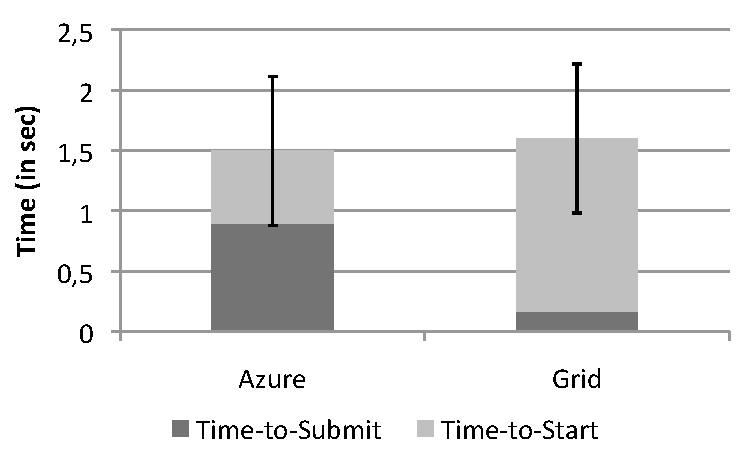
\includegraphics[width=0.4\textwidth]{performance/startup.pdf}
        \caption{BigJob Sub-Job Submission: The submission time for
          a single sub-job. The submission times to Azure and a grid
          resource are comparable. Experiments are repeated 20 times.
%           \jhanote{Is this dependent on the number of subjobs?
%             If so how many subjobs was this for?}\alnote{This was for
%             just one subjob concurrently. The experiment was repeated
%             ~20 times.  Probably the times depend on the
%             \#subjobs. Haven't had the chance to measure such times
%             yet: We probably want to use multiple threads for this
%             purpose - otherwise the times would be skewed since sj
%             submission and waiting times of the individuals sj's would
%             overlap.}\jhanote{OK. Please check my modified caption..}
%             \alnote{Reads well}
          }
    \label{fig:performance_startup}
\end{figure}

% Also,
% there is a large fluctuation in particular in the EC2 environment
% probably caused by the fact that insufficient resources were available
% at certain times.

\subsection{Ensembles on Different Resource Types}
\up
\label{sec:performance_namd}

\begin{figure}[t]
    \centering
        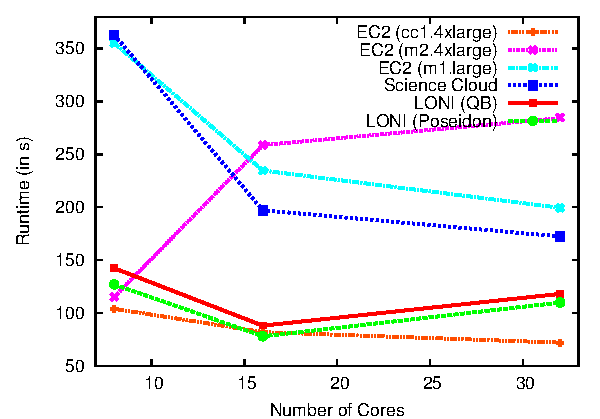
\includegraphics[width=0.4\textwidth]{performance/namd_run}
    \caption{\textbf{NAMD Runtimes on Different Resource Types: } The
          graph shows that the new EC2 cluster compute instances are 
          able to outperform other cloud resources as well as traditional
          HPC resources as QB and Poseidon. % \jhanote{this figure is
%             not referenced from/in the text anywhere!} \alnote{fixed}
          \up}
    \label{fig:performance_namd_run}

\end{figure}

% The FutureGrid Nimbus cloud is accessed via the WSRF interface,
% while for EC2 the Amazon command line client is used.

We ran experiments with NAMD in different environments with varying
characteristics: FutureGrid (Nimbus), Amazon EC2, Azure and LONI/TG.
Each FutureGrid VM provides 2 virtual cores and 3.7\,GB memory.
Amazon offers different VM types with up to 8 cores. We used, (i) the
largest VM type (m2.4xlarge) with 8 cores and 68.4\,GB of memory, (ii)
the m1.large instance type with 2 cores and 7.5\,GB, and (iii) the
recently launched cluster compute instances~\cite{ec2-cc}, which
provide a pair of quad-core Intel X5570 (Nehalem) processors with
23\,GB memory. In contrast to other instance types, cluster compute
instances are connected using 10 Gbps Ethernet. The results
of this experiment are depicted in figure~\ref{fig:performance_namd_run}
and show that cloud resources can achieve a comparable and in some cases even
a better performance than the used grid resources.


\begin{figure}[t]
    \centering
        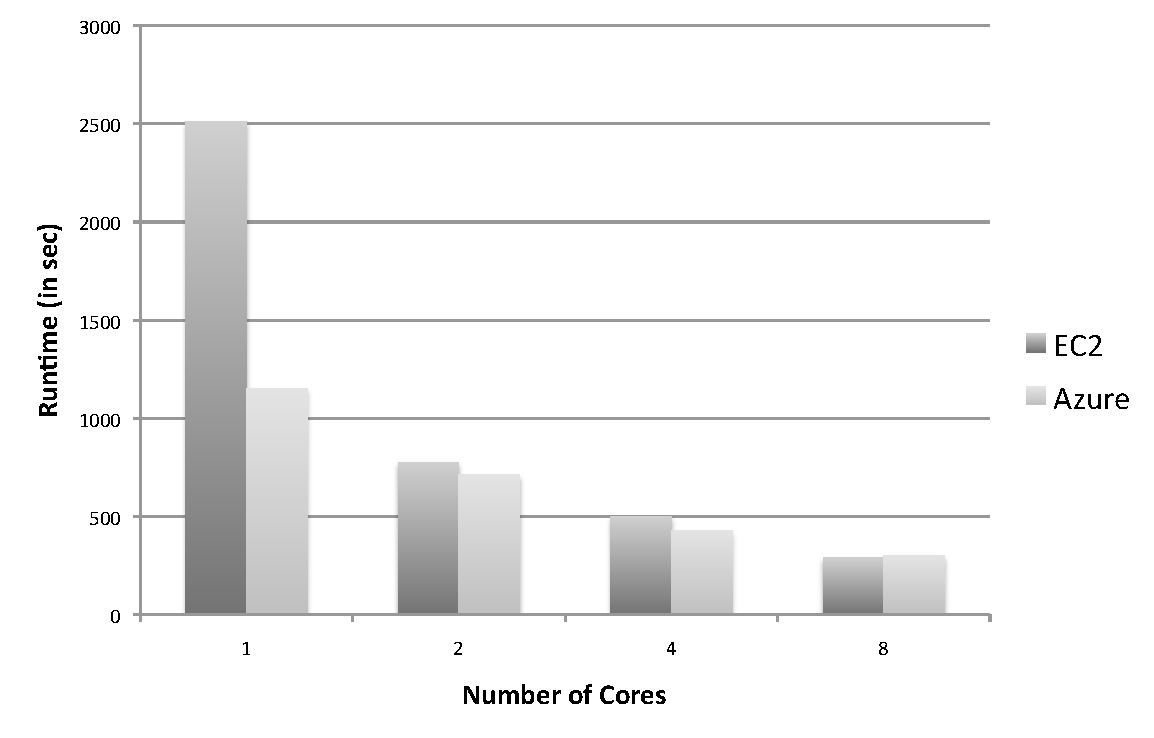
\includegraphics[width=0.4\textwidth]{performance/namd_ec2_azure.pdf}
        \up
        \caption{\textbf{NAMD Performance on Azure and EC2:} In
          particular on smaller VM sizes (1-4 cores) Azure outperforms
          EC2. The 8 core EC2 VM cc1.xlarge shows a slightly better
          performance than the Azure 8 core VM, however at a higher
          cost.} %(1.16\,\$ in comparison to 0.96\,\$).}
    \label{fig:performance_namd_ec2_azure}
\end{figure}

Figure~\ref{fig:performance_namd_ec2_azure} compares the performances
of Azure and EC2. For this purpose, an EC2 instance type with a similar core
count and price is chosen. Azure outperforms EC2 Windows instances in 
most cases; which is noteworthy, since the costs for 2, 4 and 8 core VMs are
drastically lower on Azure. Table~\ref{tbl:costs} summarizes the
costs of selected EC2 and Azure scenarios. In particular, the EC2
Linux instances show a good price/performance ratio. For Windows
instances Azure provides a favorable optimum.


% Since the underlying hardware is not known
% one can only speculate about the reason. Microsoft controls the
% hardware in its data center und optimizes its custom-built Azure
% Hypervisor with respect to this hardware~\cite{Krishnan:2010nx}, which
% could be a reason for the better performance. 

\begin{table}[ht]
    \centering
	\begin{scriptsize}
		\begin{tabular}{|l|c|c|c|c|c|}
	        \hline
	        VM Type                 &CPU h  &\#Core &\#VM &\tc &Costs  \\ \hline
	        %EC2 m1.large  (Linux)   &2          &4     &355\,sec    &0.27\$  \\ \hline
	        EC2 m2.4xlarge (Lin)  &2.40\$  &8          &1      &128\,sec     &0.08\$ \\ \hline
	        EC2 cc1.4xlarge (Lin) &1.60\$  &8          &1      &45\,sec     &0.04\$ \\ \hline
	        EC2 c1.xlarge   (Win)   &1.16\$  &8          &1      &290\,sec    &0.09\$ \\ \hline
	        Azure XL (Win)  &0.96\$ &8          &1      &301\,sec    &0.08\$ \\ \hline
		\end{tabular}
	\end{scriptsize}
	\caption{EC2 vs. Azure Costs\label{tbl:costs}}
	\up
\end{table}

\subsection{Data-Management on Azure}
\up Azure provides various options to distribute data and
compute. Users can either select one of the six data centers (as of
Sept. 2010), or a geographic region (i.\,e.\ US, Europe,
Asia). Further, Azure offers so-called affinity groups as abstractions
to control the co-location of data/compute.

To evaluate the available bandwidths and storage options, we conducted
the following experiment: a 4.3\,GB file is stored in the ABS in the
``West-EU`'' data center. This file is then downloaded by worker roles
in different locations: the same data center, ``Anywhere US'',
``Anywhere Asia'', ``Anywhere Europe'' and the same affinity group.

\begin{figure}[t]
  \centering
        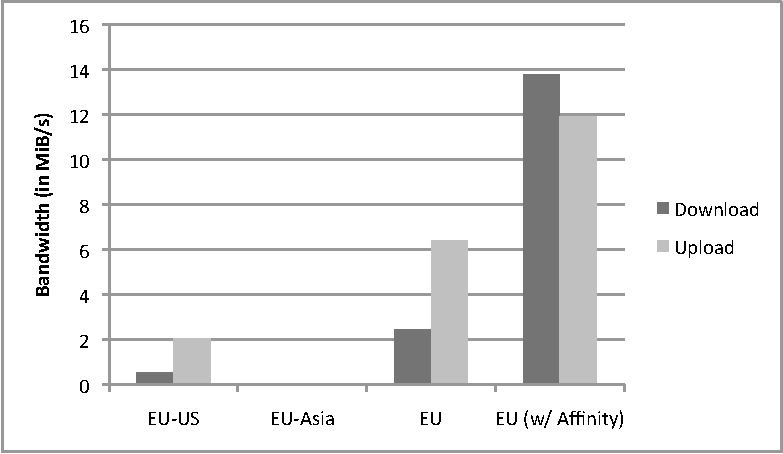
\includegraphics[width=0.4\textwidth]{performance/azure-data-transfer.pdf}
          \caption{\textbf{ABS Bandwidths Between
            Different Regions:} The achievable vary greatly with the
          distance between data and compute. Using affinity groups a
          bandwidth of approx. 12 MiB/s is achievable.}
          % , which is comparable to the bandwidth that can be achieved by manually
          % co-locating data and compute to the same data center.  }
    \label{fig:performance_azure-data-transfer}
%    \up\up
\end{figure}
Figure~\ref{fig:performance_azure-data-transfer} presents the results
of this experiment.  Obviously, the further away the worker role,
the smaller the available bandwidth. Interestingly, even when staying
in the same region (``Anywhere Europe'') the most optimal bandwidth is
not achieved.
% not the most optimal bandwidth can be
% achieved.

The best result (approx. 12 MB/s) % \jhanote{12MB/s?}
can be achieved when placing worker roles and storage in the same data
center or the same affinity group. While affinity groups provide a
good abstraction to manage compute/storage locations, it influences
the placement solely at the data-center level. The same bandwidths can
be achieved by a manual placement. Enhanced affinity groups that can
be used to control the locality on rack/switch-level would be
desirable.

% the achievable bandwidths
% are comparable to a manually placements of VMs and storage. That means 
% that Azure does not provide an option to control data locality within
% a data center.

While data locality is not critical for the EnMD and RE use case --
the Azure service package has a size of 8\,MByte, for data-intensive
applications, such as MapReduce-based applications, this is an
important feature. By supporting the Azure affinities within the
BigJob framework, these requirements can be addressed.  \up

\subsection{Replica-Exchange on Azure}
\up
\begin{figure}[t]
    \centering
        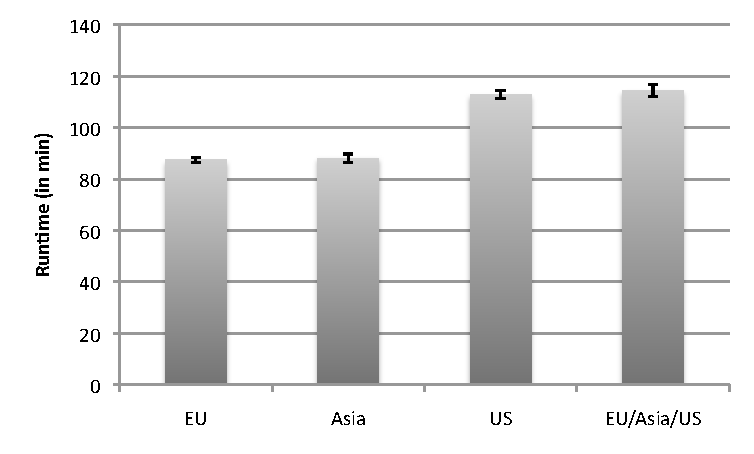
\includegraphics[width=0.4\textwidth]{performance/repex_runtime_per_region.pdf}
        \up
        \caption{\textbf{\tc for RE Run in Different Azure Regions:}
          Runtime for a RE simulation with 16 replicas each running on
          a small VM with 1 core for 500 timesteps and a total of 4
          generations. The performance of the Azure fluctuates with
          the data center region.}
        % \jhanote{Maybe legends could be made larger -- without us
        %ing more space?}
        %\up}
    \label{fig:performance_repex_runtime_per_region}
    \up
\end{figure}

Figure~\ref{fig:performance_repex_runtime_per_region} shows the
time-to-completion (\tcnsp) of an RE simulation with 16 replicas each
running on a single core VM for 500 NAMD timesteps on Azure. In total,
we measured the time for 4 generations, i.\,e.,\ for 64 attempted
exchanges. As shown in the graph, the runtime of this scenario fluctuates
with the chosen Azure region. The EU and Asia show a better
performance than the US data centers. BigJob also supports the
distribution of sub-jobs across multiple data centers. However, due to
the coupling between the replicas, the performance in this case
depends on the slowest machine.

Figure~\ref{fig:performance_repex_scaleout_vmsizes} shows \tc for
different numbers of replicas and VM types.  Again, each replica is
run for 500 timesteps before an exchange is attempted. As the number
of replicas increases, it is expected that the coordination overhead
\jhanote{I think the master here is
  infrastructure level and not application level? Need clarification
  please} \alnote{In this case I mean the application-level master
  since we are talking about the replica exchange (renamed it to
  replica master).  Of course, the overhead for the BM also
  increases.}\jhanote{OK, I see your point. Hopefully addressing thee
  earlier point about the replica master will make this clearer too}
will increase. As seen in
Figure~\ref{fig:performance_repex_scaleout_vmsizes}, this overhead for
upto 32 replicas is {\it at maximum} 2.3\,percent of the overall
runtime. \jhanote{please check} \alnote{sounds good, computed the
  overhead from my data and added it to sentence}
\begin{figure}[ht]
    \centering
        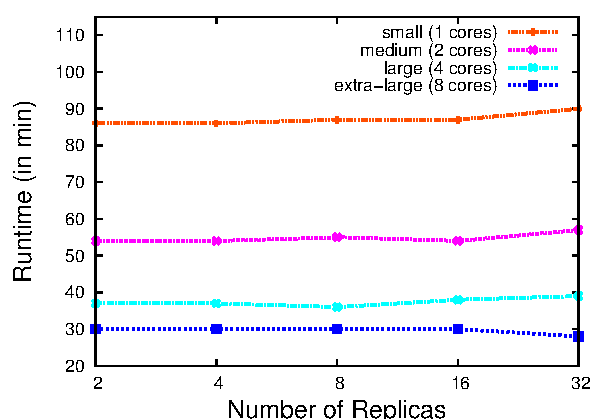
\includegraphics[width=0.4\textwidth]{performance/repex-azure.pdf}
        \caption{\textbf{\tc for Different VM Sizes and Number of
            Replicas:} With an increasing number of replicas a small
          coordination can be observed in most scenarios. The VM type
          has a great impact on the overall runtime. The larger the
          VM, the shorter \tc. }
    \label{fig:performance_repex_scaleout_vmsizes}
    \up
\end{figure}

The chosen VM type greatly influences \tcnsp. Azure currently offers
four types: small VMs with 1 core, medium VMs with 2 cores, large VMs
with 8 cores and extra-large VMs with 8 cores. The larger the VM, the
shorter the overall runtime.  However, the efficiency -- defined as,
the run-time on one resource divided by the run-time on multiple
resources scaled by the number of resources, for this problem instance
on going from the 4 to 8 cores drops to less than $0.4$. This is
mainly a limitation of the used setup: in this scenario the replicas
consist of relatively short-running NAMD tasks.  For longer-running
tasks greater efficiency can be
expected.  % \jhanote{Can you elaborate here. For example, we
%   haven't defined efficiency... The reader will find it difficult to
%   see this point}\alnote{defined efficiency and elaborated a little
%   why the efficiency is not so good.}

Nevertheless, the best performance is achieved on an extra-large
VM. The largest ensemble comprised of 32 replicas running on
extra-large VMs on a total of 256 cores.  With a runtime of
30\,minutes for the 16 replica case this setup is able to almost match
the performance of the TG resource QueenBee, where the same scenario
was executed in 26\,minutes (see~\cite{repex_ptrsb} for details).

\up
\section{Conclusion and Future Directions}
\up
% RE is a popular algorithm often used by molecular dynamics approaches
% to enhance the sampling and rate of convergence for a biological
% system.

Ensemble-based MD simulations %(enMD \& REMD)
are commonly used bio-molecular simulation
approaches. % to enhance the sampling and convergence for biomolecular
% simulations.
We have implemented the computational and coordination pattern
represented by RE to Azure, by extending the BigJob framework to
utilize the native abstractions provided by Azure, such as worker
roles, Azure storage and affinity groups.
% including the underlying BigJob framework to Azure utilizing its
% native abstractions, such as worker

In contrast to other cloud offerings, Azure provides not only
bare-metal VMs to applications, but a managed PaaS environment for
running them. It also monitors and automatically restarts VMs and
applications if necessary. Additional resources can be dynamically
spawned, e.\,g.,\ if a higher accuracy is required or a deadline must
be met. Further, Azure provides an integrated development environment
and a higher-level API, which simplifies the development considerably,
in particular compared to the efforts necessary when running an
application distributed across multiple TG sites (which to date does
not have a system-level tool for multi-site data or job
coordination). Using Azure we were able to achieve almost the same
sampling speed as on comparable grid resources, such as QueenBee.
Thus given its ``rich'' features, and simplicity invoking them, not
only is Azure a viable alternative to the TG for medium-level parallel
tasks, but it may even be the preferred alternative!

{\it Future Directions:} SAGA~\cite{saga_url} provides a simple,
single interface to the common distributed functionality (file/data,
job/VM launch etc.) for a range of distributed infrastructure.  Given
the benefit of using the same application across different
infrastructures, it makes eminent sense to support Azure from within
SAGA and to provide SAGA adaptors to important Azure services. % As
% part of ongoing research into data-intensive applications,
We are exploring novel abstractions, as well as extensions to those
already provided by Azure for data-intensive applications; we are also
investigating task placement algorithms in conjunction with different
Azure worker roles, storage and affinity group setups.
% Further, we will investigate the usage of different data-intensive
% applications (MapReduce, DAG-based applications) on
% Azure.% % SAGA is heavily used by scientific applications for distributed
% % coordination – either fine grained as in MapReduce applications, or
% % coarse-grained as in the RE case.  Given this putative benefit, it
% % makes eminent sense to support Azure from within SAGA and to provide
% % SAGA adaptors to important Azure services. 
% \jhanote{this is a candidate for shortening. maybe just focus on the
%   joint grid-cloud capability that saga-azure would
%   provide}\alnote{shortened paragraph above, merged with second
%   paragraph future work}
  
  
% Many scientific applications, e.\,g.\ DAG-based or MapReduce-based
% application involve the management of large amounts of data. In the
% future, we will further investigate different task placement
% algorithms for data-intensive applications in conjunction with
%   different Azure worker roles, storage and affinity group setups.  

  


\up
\begin{acknowledgement} 
  \up \footnotesize{% Important funding for SAGA has been provided by
%     the UK EPSRC grant number GR/D0766171/1 (via OMII-UK) and HPCOPS
%     NSF-OCI 0710874.
    SJ acknowledges the e-Science Institute, Edinburgh for supporting
    the research theme. ``Distributed Programming Abstractions'' \&
    3DPAS.  We thank J Kim (CCT) for assistance with the RNA models,
    and H Kaiser (CCT) for assistance with SAGA/Windows. We thank
    FutureGrid and Microsoft for providing the resources for the
    experiments.}
%     theme members for shaping many important ideas. This work has also
%     been made possible thanks to the internal resources of the Center
%     for Computation \& Technology at Louisiana State University and
%     computer resources provided by LONI.
\end{acknowledgement}

\up
\bibliographystyle{IEEEtran}
%\bibliography{literatur,saga,cloud,repex}
\bibliography{saga,cloud,repex}
\end{document}



